\clearpage
\begin{figure}[t!]
  \begin{center}
    \subfigure[Hadronic sample (linear scale)]{
      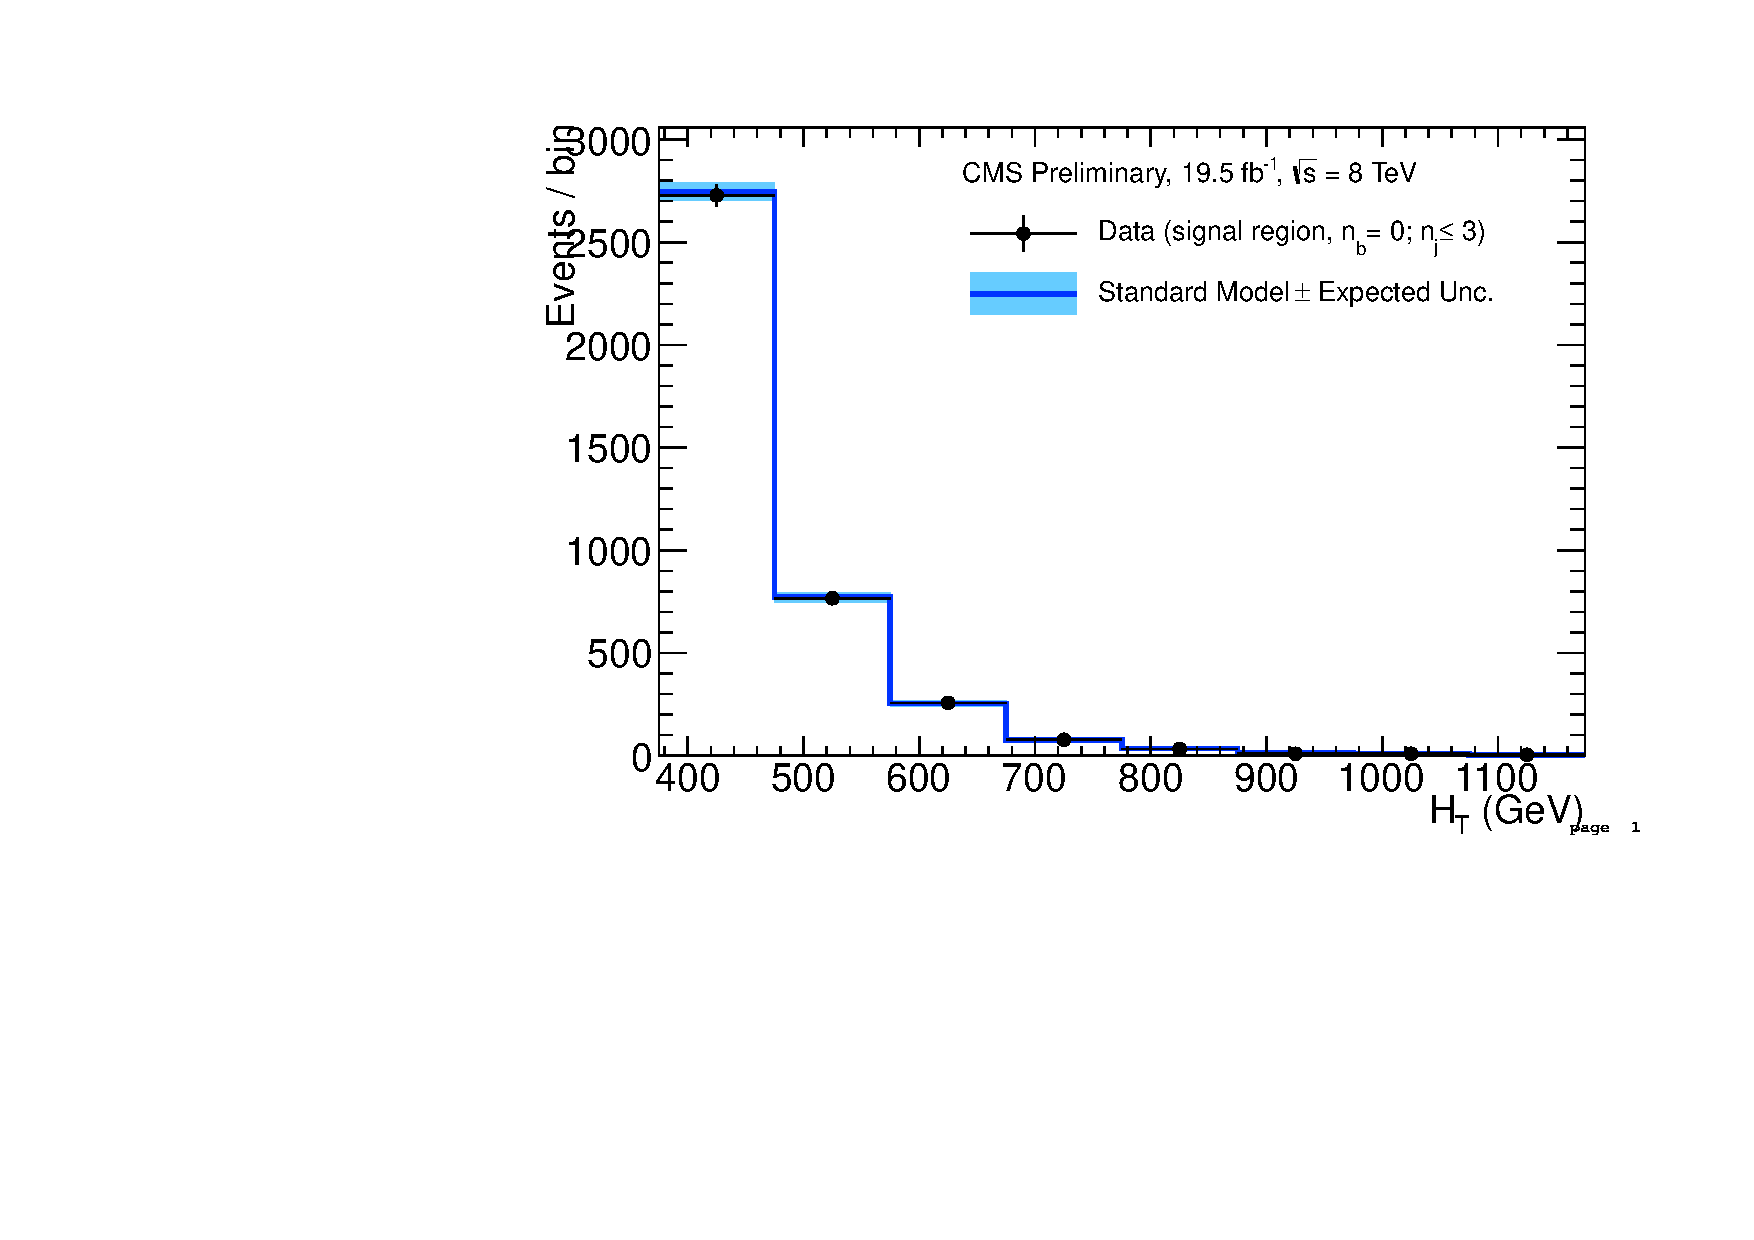
\includegraphics[width=0.45\textwidth,page=1]{figures/fit/v22/bestFit_2012pf_RQcdZero_fZinvAll_0b_le3j-1hp_smOnly}
    } 
    \subfigure[Hadronic sample (logarithmic scale)]{
      \includegraphics[width=0.45\textwidth,page=2]{figures/fit/v22/bestFit_2012pf_RQcdZero_fZinvAll_0b_le3j-1hp_smOnly}
    } \\
    \subfigure[$\mu$ + jets sample]{
      \includegraphics[width=0.45\textwidth,page=4]{figures/fit/v22/bestFit_2012pf_RQcdZero_fZinvAll_0b_le3j-1hp_smOnly}
    } 
    \subfigure[$\gamma$ + jets sample]{
      \includegraphics[width=0.45\textwidth,page=6]{figures/fit/v22/bestFit_2012pf_RQcdZero_fZinvAll_0b_le3j-1hp_smOnly}
    } 
    \caption{\label{fig:best-fit-le3j0b} Comparison of the
      \scalht-binned observed data yields and SM expectations when
      requiring \njetlow and $\nb = 0$ for the (a-b) hadronic, (c)
      \mj, (d) \mmj and (e) \gj samples, as determined by a
      simultaneous fit to all data samples under the SM-only
      hypothesis. The observed event yields in data (black dots) and
      the expectations and their uncertainties (dark blue solid line
      with light blue bands), as determined by the simultaneous fit,
      are shown. For illustrative purposes only, the signal
      expectations (pink dashed line) for the model \texttt{T2cc} with
      $m_{\sq} = 250\GeV$ and $m_{\text{LSP}} = 240\GeV$ are stacked
      on top of the SM expectations.}
  \end{center}
\end{figure}

\clearpage
\begin{figure}[t!]
  \begin{center}
    \subfigure[Hadronic sample (linear scale)]{
      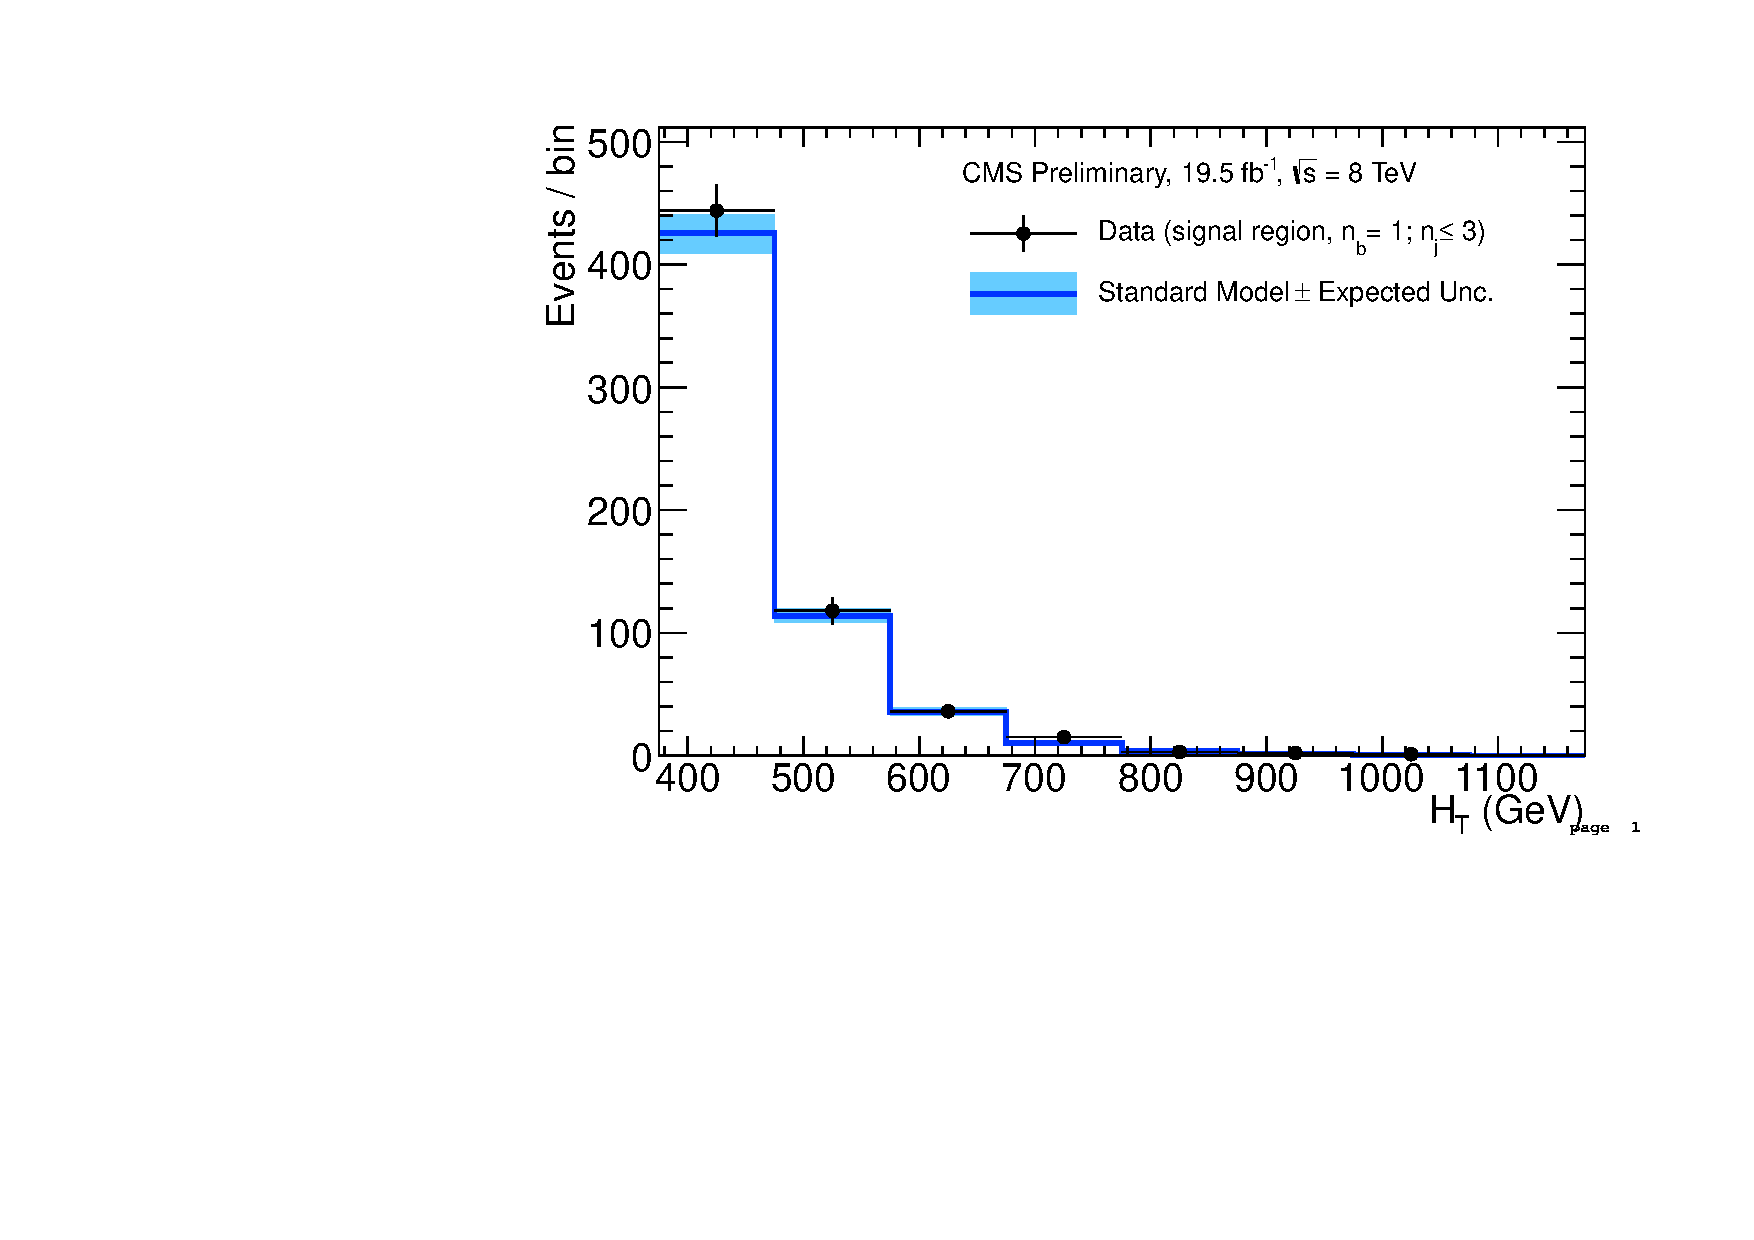
\includegraphics[width=0.45\textwidth,page=1]{figures/fit/v22/bestFit_2012pf_RQcdZero_fZinvAll_1b_le3j-1hp_smOnly}
    } 
    \subfigure[Hadronic sample (logarithmic scale)]{
      \includegraphics[width=0.45\textwidth,page=2]{figures/fit/v22/bestFit_2012pf_RQcdZero_fZinvAll_1b_le3j-1hp_smOnly}
    } \\
    \subfigure[$\mu$ + jets sample]{
      \includegraphics[width=0.45\textwidth,page=4]{figures/fit/v22/bestFit_2012pf_RQcdZero_fZinvAll_1b_le3j-1hp_smOnly}
    } 
    \subfigure[$\gamma$ + jets sample]{
      \includegraphics[width=0.45\textwidth,page=6]{figures/fit/v22/bestFit_2012pf_RQcdZero_fZinvAll_1b_le3j-1hp_smOnly}
    } 
    \caption{\label{fig:best-fit-le3j1b} Comparison of the
      \scalht-binned observed data yields and SM expectations when
      requiring \njetlow and $\nb = 1$ for the (a-b) hadronic, (c)
      \mj, (d) \mmj and (e) \gj samples, as determined by a
      simultaneous fit to all data samples under the SM-only
      hypothesis. The observed event yields in data (black dots) and
      the expectations and their uncertainties (dark blue solid line
      with light blue bands), as determined by the simultaneous fit,
      are shown. For illustrative purposes only, the signal
      expectations (pink dashed line) for the model \texttt{T2cc} with
      $m_{\sq} = 250\GeV$ and $m_{\text{LSP}} = 170\GeV$ are stacked
      on top of the SM expectations.}
  \end{center}
\end{figure}

\clearpage
\begin{figure}[t!]
  \begin{center}
    \subfigure[Hadronic sample (linear scale)]{
      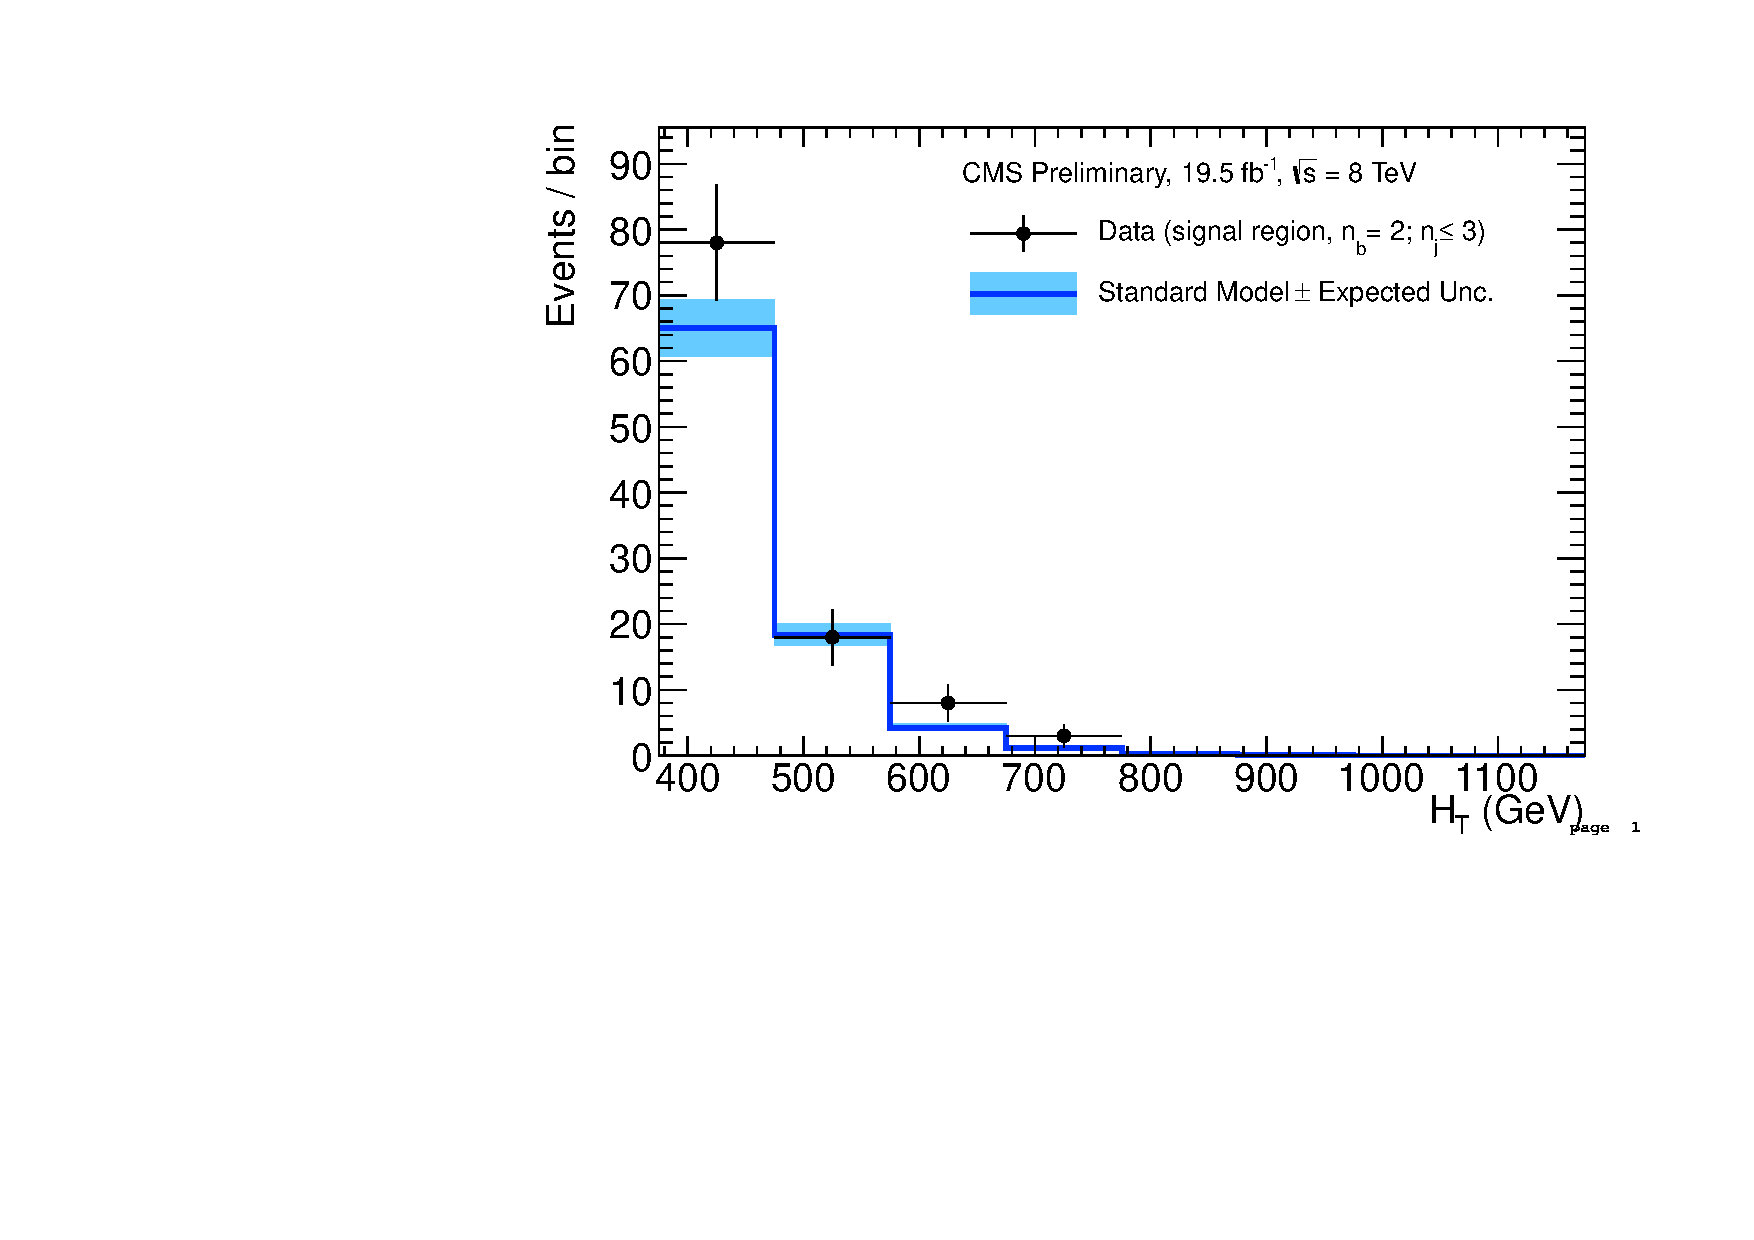
\includegraphics[width=0.45\textwidth,page=1]{figures/fit/v22/bestFit_2012pf_RQcdZero_fZinvAll_2b_le3j-1h_smOnly}
    } 
    \subfigure[Hadronic sample (logarithmic scale)]{
      \includegraphics[width=0.45\textwidth,page=2]{figures/fit/v22/bestFit_2012pf_RQcdZero_fZinvAll_2b_le3j-1h_smOnly}
    } \\
    \subfigure[$\mu$ + jets sample]{
      \includegraphics[width=0.45\textwidth,page=4]{figures/fit/v22/bestFit_2012pf_RQcdZero_fZinvAll_2b_le3j-1h_smOnly}
    } 
    \caption{\label{fig:best-fit-le3j2b} Comparison of the
      \scalht-binned observed data yields and SM expectations when
      requiring \njetlow and $\nb = 2$ for the (a-b) hadronic and \mj
      samples, as determined by a simultaneous fit to both the
      hadronic and \mj data samples under the SM-only hypothesis. The
      observed event yields in data (black dots) and the expectations
      and their uncertainties (dark blue solid line with light blue
      bands), as determined by the simultaneous fit, are shown. }
%      For illustrative purposes only, the signal expectations (pink
%      dashed line) for the model \texttt{T2cc} with $m_{\sq} =
%      250\GeV$ and $m_{\text{LSP}} = 240\GeV$ are stacked on top of
%      the SM expectations.}
  \end{center}
\end{figure}

\clearpage
\begin{figure}[t!]
  \begin{center}
    \subfigure[Hadronic sample (linear scale)]{
      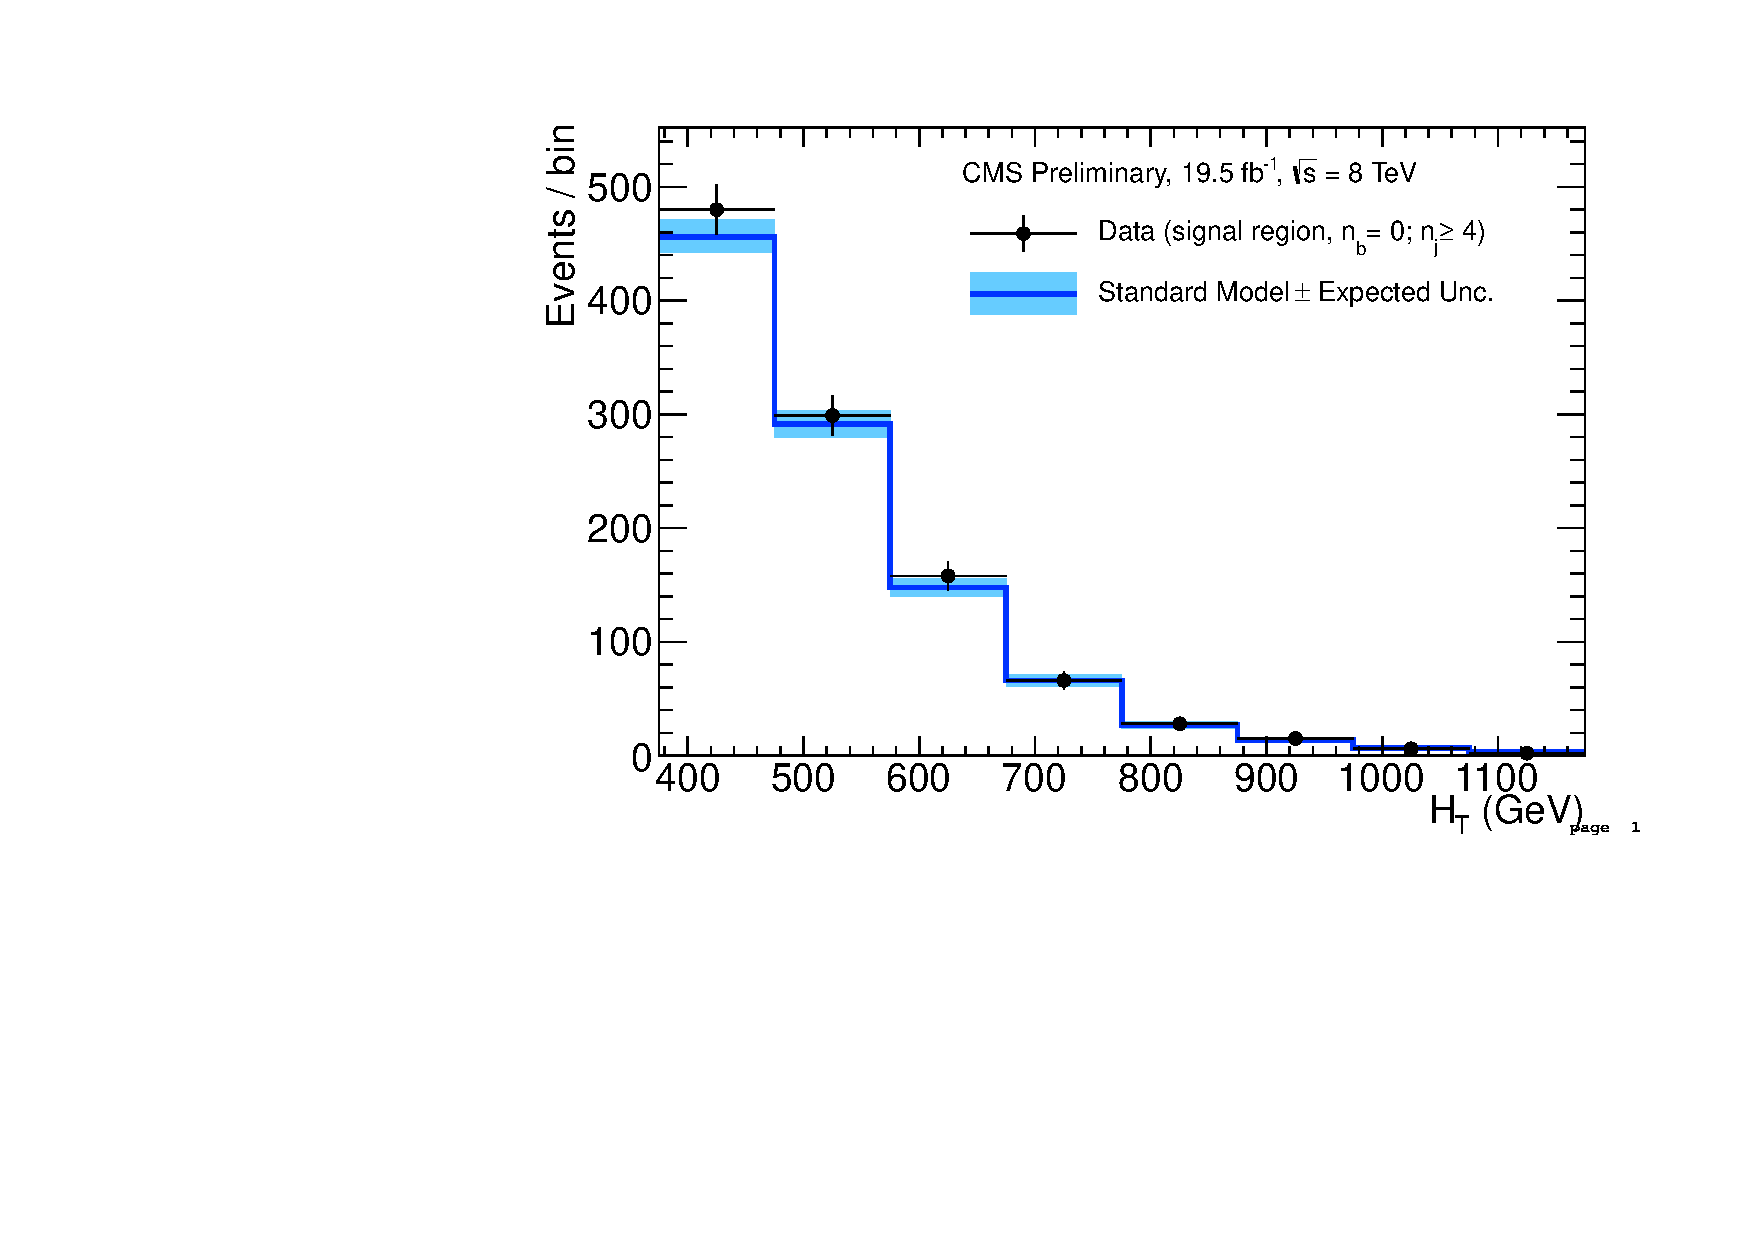
\includegraphics[width=0.45\textwidth,page=1]{figures/fit/v22/bestFit_2012pf_RQcdZero_fZinvAll_0b_ge4j-1hp_smOnly}
    } 
    \subfigure[Hadronic sample (logarithmic scale)]{
      \includegraphics[width=0.45\textwidth,page=2]{figures/fit/v22/bestFit_2012pf_RQcdZero_fZinvAll_0b_ge4j-1hp_smOnly}
    } \\
    \subfigure[$\mu$ + jets sample]{
      \includegraphics[width=0.45\textwidth,page=4]{figures/fit/v22/bestFit_2012pf_RQcdZero_fZinvAll_0b_ge4j-1hp_smOnly}
    } 
    \subfigure[$\gamma$ + jets sample]{
      \includegraphics[width=0.45\textwidth,page=6]{figures/fit/v22/bestFit_2012pf_RQcdZero_fZinvAll_0b_ge4j-1hp_smOnly}
    } 
    \caption{\label{fig:best-fit-ge4j0b} Comparison of the
      \scalht-binned observed data yields and SM expectations when
      requiring \njethigh and $\nb = 0$ for the (a-b) hadronic, (c)
      \mj, (d) \mmj and (e) \gj samples, as determined by a
      simultaneous fit to all data samples under the SM-only
      hypothesis. The observed event yields in data (black dots) and
      the expectations and their uncertainties (dark blue solid line
      with light blue bands), as determined by the simultaneous fit,
      are shown. For illustrative purposes only, the signal
      expectations (pink dashed line) for the model \texttt{T2cc} with
      $m_{\sq} = 250\GeV$ and $m_{\text{LSP}} = 170\GeV$ are stacked
      on top of the SM expectations.}
  \end{center}
\end{figure}

\clearpage
\begin{figure}[t!]
  \begin{center}
    \subfigure[Hadronic sample (linear scale)]{
      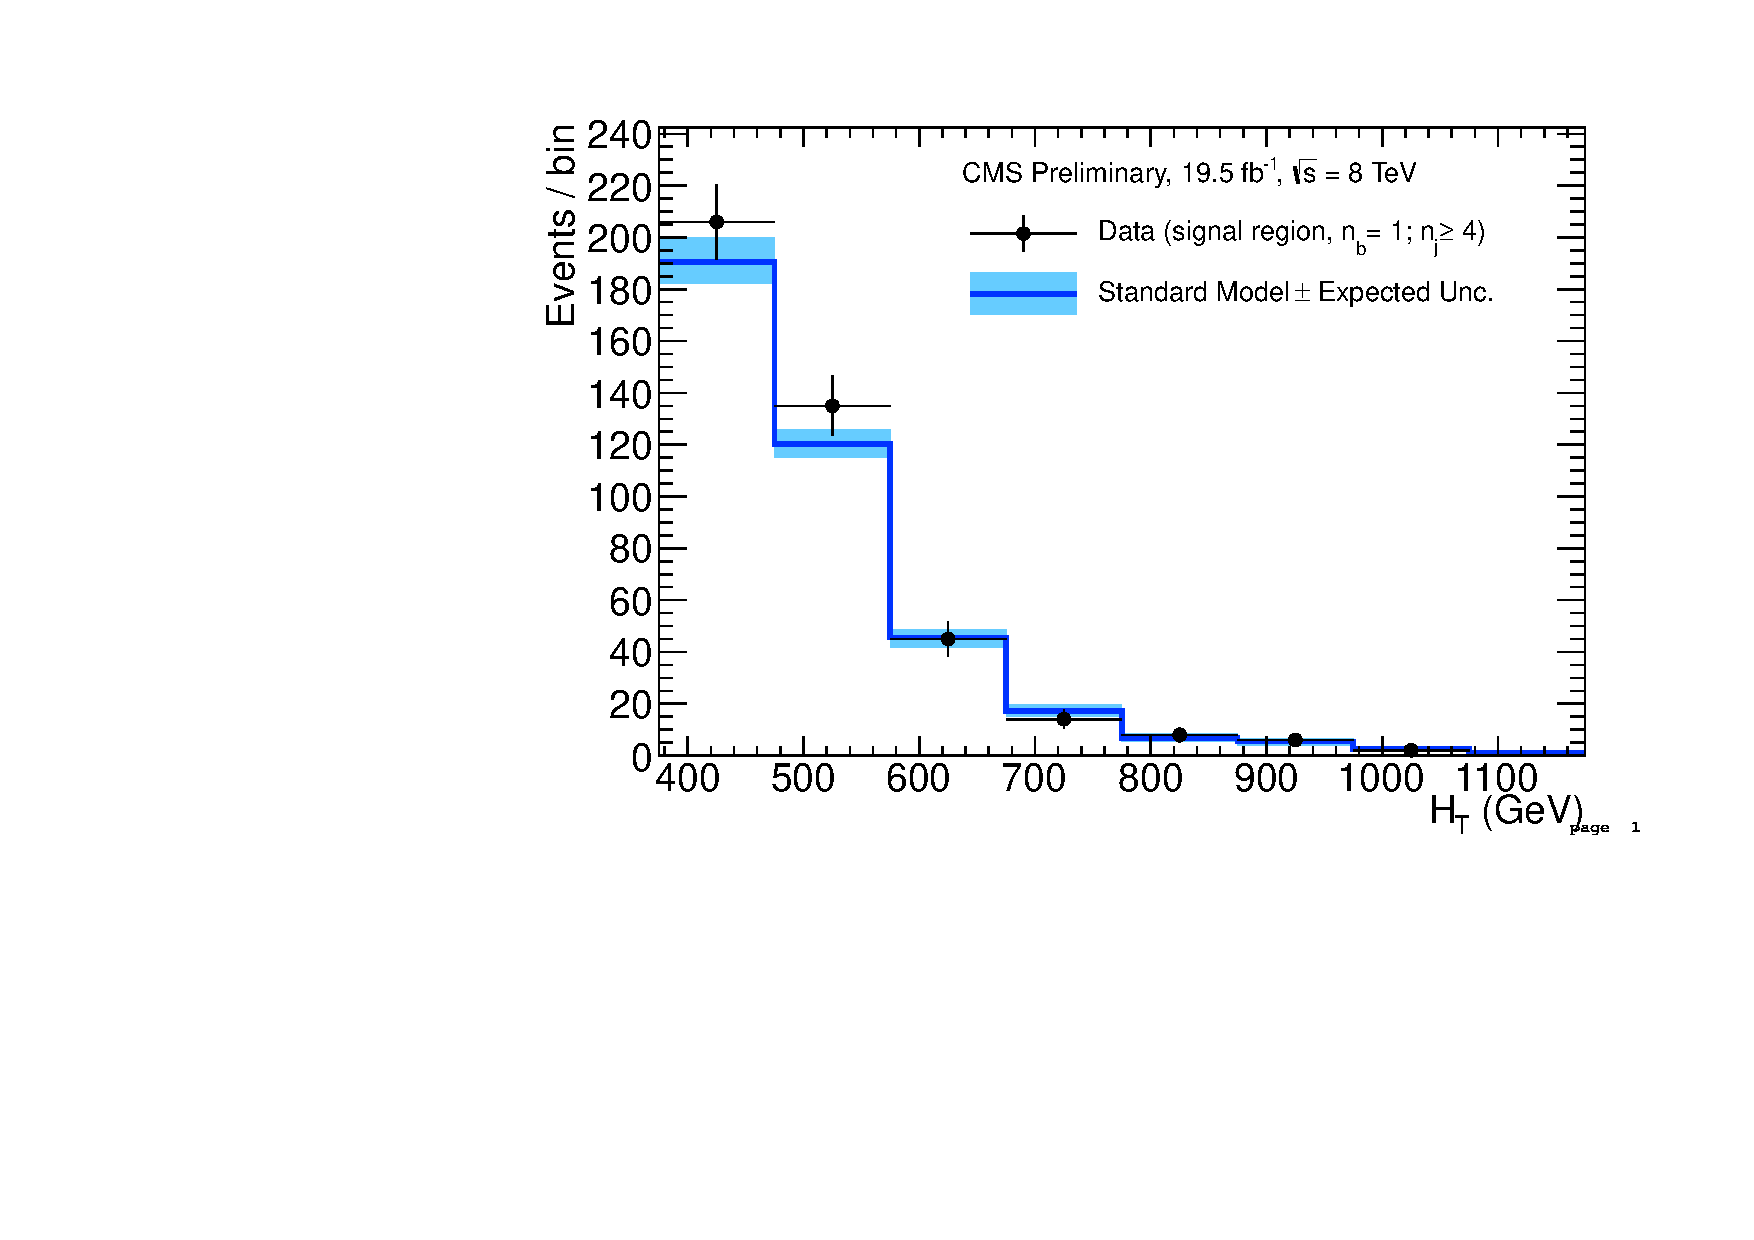
\includegraphics[width=0.45\textwidth,page=1]{figures/fit/v22/bestFit_2012pf_RQcdZero_fZinvAll_1b_ge4j-1hp_smOnly}
    } 
    \subfigure[Hadronic sample (logarithmic scale)]{
      \includegraphics[width=0.45\textwidth,page=2]{figures/fit/v22/bestFit_2012pf_RQcdZero_fZinvAll_1b_ge4j-1hp_smOnly}
    } \\
    \subfigure[$\mu$ + jets sample]{
      \includegraphics[width=0.45\textwidth,page=4]{figures/fit/v22/bestFit_2012pf_RQcdZero_fZinvAll_1b_ge4j-1hp_smOnly}
    } 
    \subfigure[$\gamma$ + jets sample]{
      \includegraphics[width=0.45\textwidth,page=6]{figures/fit/v22/bestFit_2012pf_RQcdZero_fZinvAll_1b_ge4j-1hp_smOnly}
    } 
    \caption{\label{fig:best-fit-ge4j1b} Comparison of the
      \scalht-binned observed data yields and SM expectations when
      requiring \njethigh and $\nb = 1$ for the (a-b) hadronic, (c)
      \mj, (d) \mmj and (e) \gj samples, as determined by a
      simultaneous fit to all data samples under the SM-only
      hypothesis. The observed event yields in data (black dots) and
      the expectations and their uncertainties (dark blue solid line
      with light blue bands), as determined by the simultaneous fit,
      are shown. For illustrative purposes only, the signal
      expectations (pink dashed line) for the model \texttt{T2cc} with
      $m_{\sq} = 250\GeV$ and $m_{\text{LSP}} = 170\GeV$ are stacked
      on top of the SM expectations.}
  \end{center}
\end{figure}

\clearpage
\begin{figure}[t!]
  \begin{center}
    \subfigure[Hadronic sample (linear scale)]{
      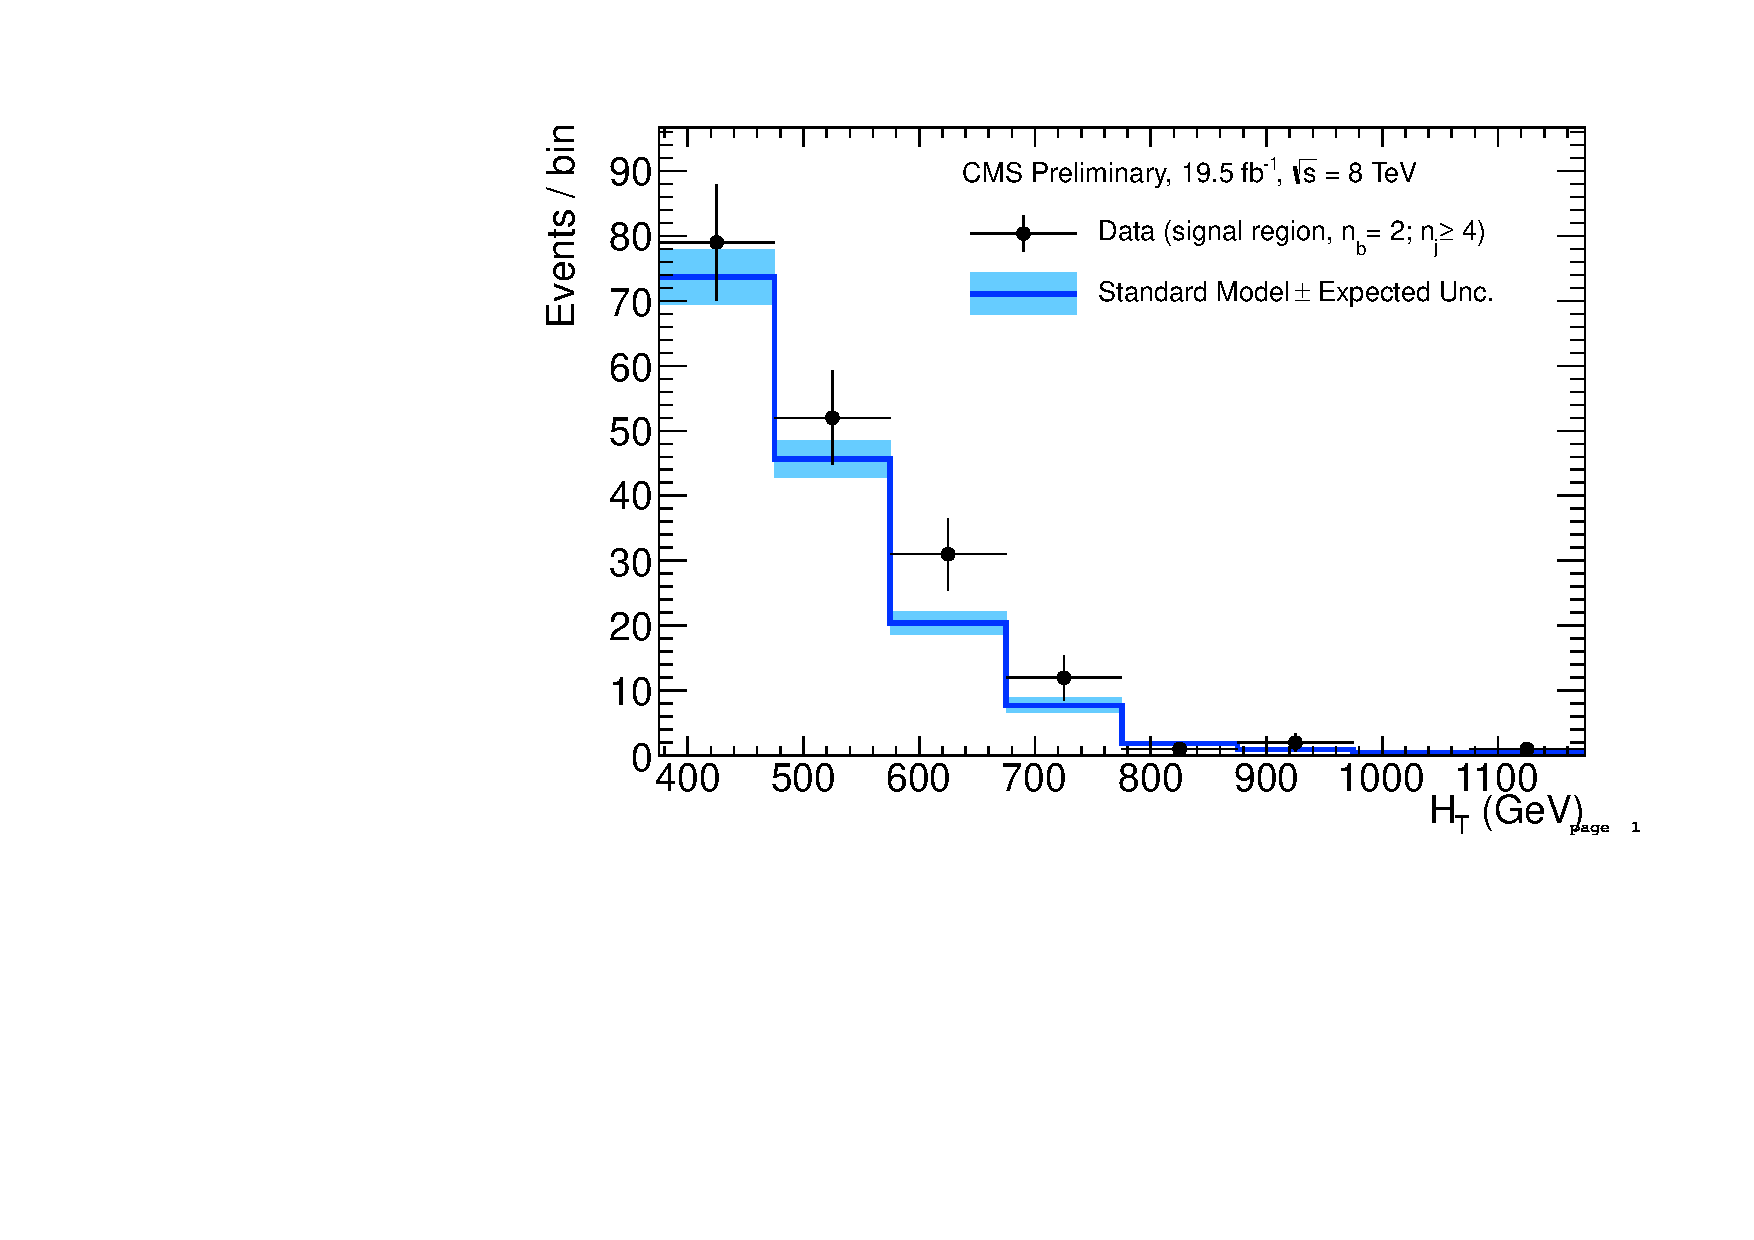
\includegraphics[width=0.45\textwidth,page=1]{figures/fit/v22/bestFit_2012pf_RQcdZero_fZinvAll_2b_ge4j-1h_smOnly}
    } 
    \subfigure[Hadronic sample (logarithmic scale)]{
      \includegraphics[width=0.45\textwidth,page=2]{figures/fit/v22/bestFit_2012pf_RQcdZero_fZinvAll_2b_ge4j-1h_smOnly}
    } \\
    \subfigure[$\mu$ + jets sample]{
      \includegraphics[width=0.45\textwidth,page=4]{figures/fit/v22/bestFit_2012pf_RQcdZero_fZinvAll_2b_ge4j-1h_smOnly}
    } 
    \caption{\label{fig:best-fit-ge4j2b} Comparison of the
      \scalht-binned observed data yields and SM expectations when
      requiring \njethigh and $\nb = 2$ for the (a-b) hadronic and \mj
      samples, as determined by a simultaneous fit to both the
      hadronic and \mj data samples under the SM-only hypothesis. The
      observed event yields in data (black dots) and the expectations
      and their uncertainties (dark blue solid line with light blue
      bands), as determined by the simultaneous fit, are shown. }
%      For illustrative purposes only, the signal expectations (pink
%      dashed line) for the model \texttt{T2cc} with $m_{\sq} =
%      250\GeV$ and $m_{\text{LSP}} = 240\GeV$ are stacked on top of
%      the SM expectations.}
  \end{center}
\end{figure}


%\clearpage
%\begin{figure}[t!]
%  \begin{center}
%    \subfigure[Hadronic sample (linear scale)]{
%      \includegraphics[width=0.45\textwidth,page=1]{figures/fit/v22/bestFit_2012pf_RQcdZero_fZinvAll_3b_ge4j-1h_smOnly}
%    } 
%    \subfigure[Hadronic sample (logarithmic scale)]{
%      \includegraphics[width=0.45\textwidth,page=2]{figures/fit/v22/bestFit_2012pf_RQcdZero_fZinvAll_3b_ge4j-1h_smOnly}
%    } \\
%    \subfigure[$\mu$ + jets sample]{
%      \includegraphics[width=0.45\textwidth,page=4]{figures/fit/v22/bestFit_2012pf_RQcdZero_fZinvAll_3b_ge4j-1h_smOnly}
%    } 
%    \caption{\label{fig:best-fit-ge4j3b} Comparison of the
%      \scalht-binned observed data yields and SM expectations when
%      requiring \njethigh and $\nb = 3$ for the (a-b) hadronic and \mj
%      samples, as determined by a simultaneous fit to both the
%      hadronic and \mj data samples under the SM-only hypothesis. The
%      observed event yields in data (black dots) and the expectations
%      and their uncertainties (dark blue solid line with light blue
%      bands), as determined by the simultaneous fit, are shown. }
%%      For illustrative purposes only, the signal expectations (pink
%%      dashed line) for the model \texttt{T2cc} with $m_{\sq} =
%%      250\GeV$ and $m_{\text{LSP}} = 240\GeV$ are stacked on top of
%%      the SM expectations.}
%  \end{center}
%\end{figure}
%
%
%\clearpage
%\begin{figure}[t!]
%  \begin{center}
%    \subfigure[Hadronic sample (linear scale)]{
%      \includegraphics[width=0.45\textwidth,page=1]{figures/fit/v22/bestFit_2012pf_RQcdZero_fZinvAll_ge4b_ge4j-1h_smOnly}
%    } 
%    \subfigure[Hadronic sample (logarithmic scale)]{
%      \includegraphics[width=0.45\textwidth,page=2]{figures/fit/v22/bestFit_2012pf_RQcdZero_fZinvAll_ge4b_ge4j-1h_smOnly}
%    } \\
%    \subfigure[$\mu$ + jets sample]{
%      \includegraphics[width=0.45\textwidth,page=4]{figures/fit/v22/bestFit_2012pf_RQcdZero_fZinvAll_ge4b_ge4j-1h_smOnly}
%    } 
%    \caption{\label{fig:best-fit-ge4jge4b} Comparison of the
%      \scalht-binned observed data yields and SM expectations when
%      requiring \njethigh and $\nb \geq 4$ for the (a-b) hadronic and \mj
%      samples, as determined by a simultaneous fit to both the
%      hadronic and \mj data samples under the SM-only hypothesis. The
%      observed event yields in data (black dots) and the expectations
%      and their uncertainties (dark blue solid line with light blue
%      bands), as determined by the simultaneous fit, are shown. }
%%      For illustrative purposes only, the signal expectations (pink
%%      dashed line) for the model \texttt{T2cc} with $m_{\sq} =
%%      250\GeV$ and $m_{\text{LSP}} = 240\GeV$ are stacked on top of
%%      the SM expectations.}
%  \end{center}
%\end{figure}
